%This document is a preview lecture for college class: Mathematical History.
%I'm a student majoring in Mathematics in China university.
%This article must has lots of shortcomings, and I sincerely invite collegues and friends to criticize, correct it.

\documentclass{Math_Note}

\title{Mathematical History(CN)}
\author{Buce-Ithon}
\newdateformat{mydate}{\twodigit{\THEDAY}{ }\shortmonthname[\THEMONTH], \THEYEAR}
\date{\today}

\begin{document}

%Title page
\maketitle

%content
\newpage
\tableofcontents
\newpage

%Chapter 1
\section{数学史——人类文明史的重要篇章}
数学史研究数学概念、数学方法和数学思想的起源和发展,及其与社会、政治、经济和一般文化的联系.
\subsection{数学史的意义}
数学作为一门发展历程几乎贯穿了人类发展史的学科,其历史性或者说积累性极强,在人类整个文明史上有着特殊的地位.
这种地位,是由数学作为一种文化的特点决定的:
\begin{itemize}
    \item 抽象性(追求高的精确、可靠的知识)
    \item 一般性(追求世界规则最大限度的一般性模式的倾向)
    \item 创造性(艺术特色)
\end{itemize}
数学是各个时代人类文明的标志之一,是了解整个人类文明史的重要渠道.
\subsection{什么是数学——历史的理解}
古希腊哲学家亚里士多德:“数学是量的科学”.

恩格斯:“数学是研究现实世界的空间形式与数量关系的科学”.

前苏联数学家:“现代数学就是各种量之间的可能的,一般说是各种变化着的量的关系与相互联系的数学”.

20世纪80年代开始,一批美国学者:“数学这个领域已被称作模式的科学(science of pattern),其目的是要解释人们从自然界和数学本身的抽象世界中所观察到的结构和对称性”.
\subsection{关于数学史的分期}
通常来说,数学史的分期线索如下:
\begin{itemize}
    \item 按时代顺序
    \item 按数学对象、方法等本身的质变过程
    \item 按数学发展的社会背景
\end{itemize}

本书(《数学史概论》)综合上述线索,作出数学史的如下分期:
\begin{enumerate}
    \item 数学的起源与早期发展 (公元前 6 世纪前)
    \item 初等数学时期 (公元前 6 世纪–16 世纪)
    \begin{enumerate}
        \item 古代希腊数学 (公元前 6 世纪–6 世纪)
        \item 中世纪东方数学 (3 世纪–15 世纪)
        \item 欧洲文艺复兴时期 (15 世纪–16 世纪)
    \end{enumerate}
    \item 近代数学时期 (或称变量数学建立时期, 17 世纪–18 世纪)
    \item 现代数学时期 (1820'–现在)
    \begin{enumerate}
        \item 现代数学酝酿时期 (1820'-1870')
        \item 现代数学形成时期 (1870'-1940')
        \item 现代数学繁荣时期 (或称当代数学时期, 1950'–现在)
    \end{enumerate}
\end{enumerate}

%Chapter 2
\section{数学的起源与早期发展}
\subsection{数与形概念的产生}
\subsubsection{初等算术}
早期人类识别事物多寡的能力促进了抽象的“数”的概念的产生。而“数”的诞生也促成了计数的需求和发展.

计数历史:手指计数$\rightarrow$石子计数$\rightarrow$结绳计数、刻痕计数$\rightarrow$书写计数与计数系统

计数系统:古埃及的象形数字(公元前3400年左右),巴比伦楔形数字(公元前2400年左右),中国甲骨文数字(公元前1600年左右),
希腊阿提卡数字(公元前500年左右),中国筹算数码(公元前500年左右),印度婆罗门数字(公元前300年左右),玛雅数字(?)

其中,除巴比伦楔形数字采用六十进制、玛雅数字采用二十进制以外,其他均属十进制数系.

\subsubsection{初等几何}
与算术相仿,最初的几何知识是从人们对形的直觉中萌发出来的.

\begin{itemize}
    \item 古希腊学者希罗多德(Herodotus, 约公元前484~前425)研究:古埃及几何学的起源产生于尼罗河泛滥后土地的重新测量. 
    “几何学”一词的希腊文γεωμετρία意即“测地”.
    \item 古代印度几何学的起源则与宗教实践密切相关:公元前8世纪至公元前5世纪形成的所谓“绳法经”,
    记载了关于祭坛和寺庙建造中的几何问题和求解法则.
    \item 古代中国:几何学更多地与天文观测相联系,流传下来的经典著作有《周髀算经》、《九章算术》(后者多被认为是中国古代算术经典)等.
\end{itemize}

\subsection{河谷文明和早期数学}
历史学家往往把兴起于埃及、美索不达米亚、中国和印度等地域的古代文明称为“ 河谷文明”.
\subsubsection{埃及数学}
埃及象形文字(hieroglyphic, 意为“ 圣刻”——神圣的雕刻)产生于公元前3500年左右,约公元前2500 年被简化为一种更易书写的“僧侣文 ”(hieratic) ,后又发展成所谓“通俗文 ”(domotic).

古埃及人在一种用纸莎草(Papyrus)压制成的草片上书写,这些纸草书有的幸存至今. 关于古埃区数学的知识,主要就是依据了两部用僧侣文写就的纸草书——莱茵德纸草书和莫斯科纸草书. 

(有趣的是,两部纸草书虽然均出自于埃及,然而由于历史原因,均流传到国外,最终以埃及以外的其他地区命名)

两部纸草书实际上都是各种类型的数学问题集:莱茵德纸草书主体由84个问题组成,莫斯科纸草书包括了25个问题.

此外,埃及人很早就发明了象形文字记号,这是一种以十进制为位值的系统,但却没有进位的概念. 这种计数制用不同的特殊记号分别表示10的前六次幂. 如下图所示:

\begin{figure}[H]
    \centering
    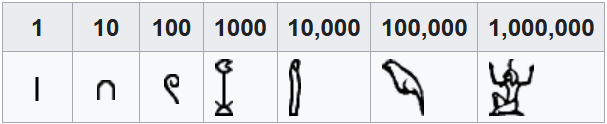
\includegraphics[scale=0.8]{"./Figures/Ancient_Egyptian_Math_1.png"} %[scale=xxx]-->[height=xxx, width=xxx]
    \caption{古埃及计数系统-10的幂次}
\end{figure}

石器时代的人未留下使用分数的痕迹,但随着更先进的青铜文化的崛起,分数概念与分数记号也应运而生.
埃及象形文字用一种特殊的记号来表示单位分数即分子为1的分数:

\begin{figure}[H]
    \centering
    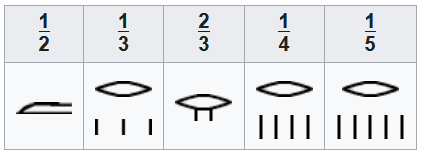
\includegraphics[scale=0.8]{"./Figures/Ancient_Egyptian_Math_2.png"}
    \caption{古埃及计数系统-分数}
\end{figure}

单位分数在埃及数学中扮演着重要的角色. 埃及人将所有的真分数都表示为一些单位分数的和($\frac{2}{3}$除外).
埃及人为什么对单位分数情有独钟,原因尚不清楚. 但是利用单位分数,分数的四则运算就可以进行,尽管过程十分麻烦.

古埃及的算术运算:加法(基础) $\rightarrow$ 乘法(逐次倍加) $\rightarrow$ 除法(乘法逆运算)

纸草书中记载了埃及人的一些计算技巧以及一部分代数学问题(如求解含未知数的一次方程).

古埃及几何学:古埃及几何学来源于埃及人对尼罗河沿岸的土地测量,现存纸草书中还能找到古埃及人对一些规则多边体以及圆面积的计算公式.

总结:埃及数学是实用数学,涉及证明较少. 与埃及文明的发展相似,埃及数学在数千年的岁月中变化很少——计算显得十分笨重、实用几何也逐渐因为忽视精确程度而带上笨重的色彩.
这一切都阻碍了埃及数学向更高的水平发展,并在公元前4世纪希腊人征服埃及后,逐渐完全被更先进的希腊数学所取代.

\subsubsection{美索不达米亚数学}
文明历史:美索不达米亚平原位于底格里斯河与幼发拉底河孕育的两河流域,由于该区域是四面开放的新月沃土带,长期以来存在着错综复杂的民族战乱.

文字:楔形文字与泥版文书(如著名的普林顿322).

计数制度:60进制(对60以内的整数采用简单十进制累计法). 此外,他们还将位值原理巧妙推广到了分数(类比于现在二进制的权值表示). 

数学方法的进步之处:计算的程序化算法;各式数表的运用;二次甚至三次方程的研究;萌发了理论研究的兴趣.

不足之处:和古埃及相似的实用几何学,停留在近似层面,精确程度不高.

总结:古代美索不达米亚数学与埃及数学一样主要是解决各类具体问题的实用知识,处于原始算法积累时期.
几何学作为一门独立的学问甚至还不存在.埃及纸草书和巴比伦泥版文书中汇集的各种几何图形面积、体积的计算法则,本质上属于算术的应用.
当然,古代实用算法积累到一定阶段,对它们进行系统整理与理论概括必然形成趋势,但这一任务并不是由早期河谷文明本身来担当的.
向理论数学的过渡,是大约公元前6世纪在地中海沿岸开始的,那里一个崭新的、更加开放的文明——历史学家常称“海洋文明”,带来
了初等数学的第一个黄金时代——以论证几何为主的希腊数学时代.

%Chapter 3
\section{古希腊数学}
希腊数学:公元前600年到公元600年间,大致范围为希腊半岛、爱琴海区域、马其顿与色雷顿地区、意大利半岛、小亚细亚及非洲北部.
\subsection{论证数学的发端}
\subsubsection{泰勒斯与毕达哥拉斯}
\textbf{泰勒斯}(Thales of Miletus, 约公元前625-前547):目前所知最早的希腊数学家,其领导的爱奥尼亚学派据称开创了希腊命题证明之先河.

学术成就:关于Thales的学术成就基本只能依靠后人(主要是公元5世纪新柏拉图派哲学家Proclus)的记载:
据说Thales曾证明了下列四条定理:
\begin{itemize}
    \item 圆的直径将圆分为两个相等的部分
    \item 等腰三角形两底角相等
    \item 两相交直线形成的对顶角相等
    \item 如果一三角形有两角、一边分别于另一三角形的对应角、边相等,那么这两个三角形全等
\end{itemize}
传说Thales还证明了“泰勒斯定理”的命题:半圆上的圆周角是直角;测量过金字塔高;预报了公元前585年的一次日食等等.

\textbf{毕达哥拉斯}(Pythagoras of Samos, 约公元前580-前500):希腊论证数学的另一位祖师,和Thales一样都没有著作留世,创建了毕达哥拉斯学派,
致力于哲学和数学的研究. 同样地,对Pythagoras生平的了解也只能从后人的记载中寻找.

逸事:相传“哲学”(φιλοσοφία)和“数学”(μαθηματικά)两个词正是Pythagoras本人所创.

学术成就:
\begin{itemize}
    \item 继Thales之后,将数学改造为自由的教育形式,首先检验其原理,并用一种无形和理智的方式探讨其定理.
    \item 据说欧几里得《原本》前二卷的大部分材料来源于毕达哥拉斯学派,包括毕达哥拉斯定理等.
    \item 此外毕达哥拉斯学派还研究了正多面体作图,他们称正多面体为“宇宙形”. 
    我们今天知道在三维空间中正多面体仅有五种一正四面体、正六面体、正八面体、正十二面体和正三十面体.
\end{itemize}

学派信条:万物皆数(这里的数指整数).

Interesting things: 
1.毕达哥拉斯学派关于“形数”的研究,强烈地反映了他们将数作为几何思维元素的精神.
\begin{figure}[H]
    \centering
    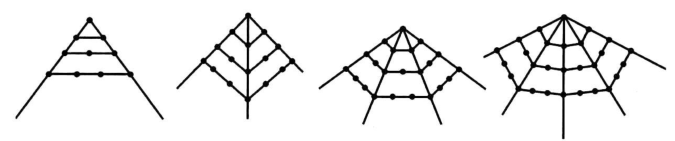
\includegraphics[scale=1.0]{"./Figures/Polygonal_number.png"}
    \caption*{多边形数}
\end{figure}
2.Pythagoras三元数组(与勾股定理密切相关):$\frac{m^{2}-1}{2},m,\frac{m^{2}+1}{2}$. 不过,这一公式并未给出所有的Pythagoras三元数组. 
3.Pythagoras相信任何一个量均可表示成两个整数之比(即一个有理量).(在无理数被发现时,这一信条引发了“第一次数学危机”)

\subsubsection{雅典时期的希腊数学}
结束了以毕达哥拉斯学派为代表的倾向于贵族制的学派,希腊数学走向了更为民主繁荣的道路. 

主要学派:
\begin{itemize}
    \item \textbf{伊利亚学派}: 芝诺(Zeno, 公元前490-前430) 德谟克里特(Democritus)的原子论学派
    \item \textbf{诡辩学派}: 希比阿斯(Hippias) 安提丰(Antiphon) 布里松(Bryson)等等
    \item \textbf{雅典学院(柏拉图学派)}: 柏拉图(Plato, 公元前427-前347) 梅内赫摩斯(Menaechmus) 狄诺斯特拉图斯(Dinostratus) 蒂奥泰德(Theaetetus) 欧多克斯(Eudoxus)
    \item \textbf{亚里士多德学派}: 亚里士多德(Aristotle, 公元前384-前322)
\end{itemize}
这些学派中的不少代表人物都曾师从Pythagoras学派或相互学派的学者.

他们的探讨活动对数学研究的推动主要表现在以下三个方面:
\begin{enumerate}
    \item 三大几何问题
    \begin{enumerate}
        \item 化圆为方,即作一个与给定的圆面积相等的正方形
        \item 倍立方体,即求作一立方体,使其体积等于已知立方体的两倍
        \item 三等分角,即分任意角为三等分
    \end{enumerate}
    \item 无限性概念的早期探索:Zeno悖论
    \item 逻辑演绎结构的倡导
\end{enumerate}

这一时期一个重要数学思想:穷竭法(可以严格证明已知命题,却不能用来发现新的结果).

\subsection{黄金时代——亚历山大学派}
从公元前338年希腊诸邦被马其顿控制,至公元前30年最后一个希腊化国家托勒密王国被罗马消灭,这三百年史称希腊数学的“黄金时代”.
这一时期,希腊数学从雅典转移到了亚历山大城,这一时期的学者也称亚历山大学派.
\subsubsection{欧几里得与《原本》}
欧几里得(Euclid of Alexandria)是希腊论证几何学的集大成者.

名言逸事:几何无王者之道.

“原本”的希腊文Στοιχεῖα(Stoicheia),原意是指一学科中具有广泛应用的最重要的定理.欧几里得在这本原著中用公理法对当时的数学知识作了系统化、理论化的总结.
全书共分13卷,包括有5条公理、5条公设、119个定义和465条命题,构成了历史上第一个数学公理体系.

《原本》共分为13卷:第一卷至第六卷的内容主要为平面几何,第七卷至第九卷主要阐述了数论,第十卷讨论了无理数,
第十一卷至第十三卷主要讨论立体几何,内容极为丰富.

以下以第一卷的5条公设和公理举例展示:
\begin{itemize}
    \item 公设
    \begin{enumerate}
        \item 假定从任意一点到任意一点可作一直线.
        \item 一条有限直线可不断延长.
        \item 以任意中心和直径可以画圆.
        \item 凡直角都彼此相等.
        \item 若一直线落在两直线上所构成的同旁内角和小于两直角,那么把两直线无限延长,
        它们将在同旁内角和小于两直角的一侧相交.
    \end{enumerate}
    \item 公理
    \begin{enumerate}
        \item 等于同量的量彼此相等.
        \item 等量加等量,和相等.
        \item 等量减等量,差相等.
        \item 彼此重合的图形是全等的.
        \item 整体大于部分.
    \end{enumerate}
\end{itemize}

毫无疑问,Euclid的《原本》奠定了后世两千余年的几何、数论以及逻辑演绎科学的不朽基础.

\subsubsection{阿基米德的数学成就}
阿基米德(Archimedes,公元前287一前212)出生于西西里岛的叙拉古(Syracuse),早年曾在亚历山大城跟过欧几里得的门生学习,后来虽然离开了亚历山大,
但仍与那里的师友保持着密切联系.他的许多成果都是通过与亚历山大学者的通信而保存下来.因此,阿基米德通常被看成是亚历山大学派的成员.

阿基米德著述极为丰富,但多以类似论文手稿而非大部巨著的形式出现.这些著述内容涉及数学、力学及天文学等. 如:
《圆的度量》(Measurement of Circle)、《论球和圆柱》(On the Sphere and Cylinder)、《论平面图形的平衡或其重心》(On the Equilibrium of Planes 
or the Centres of Gravity of Planes)、《处理力学问题的方法》(The Method Treating of Mechanical Problems)等.

阿基米德创造了“平衡法”:将需要求积的量(面积、体积等)分成许多微小单元(如微小线段、薄片等),再用另一组微小单元来进行比较,而后一组微小单元的总和比较容易计算.
只不过这两组微小单元的比较是借助于力学上的杠杆平衡原理来实现的.因此,平衡法体现了近代积分法的基本思想,可以说是阿基米德数学研究的最大功绩.阿基米德本人用它解决了
一系列几何图形的面积、体积计算问题.

当然,平衡法本身必须以极限论为基础,阿基米德意识到他的方法在严密性上的不足,所以当他用平衡法求出一个面积或体积之后,必再用穷竭法给以严格的证明.
这种发现与求证的双重方法,是阿基米德独特的思维模式,也可以说是他胜欧几里得一筹之处.

逸事与结局:“阿基米德原理”(物体在流体中所受浮力等于其派去流体的重量)的发现;阿基米德之死与他的墓碑(球及其外切圆柱).

\subsubsection{阿波罗尼斯与圆锥曲线论}
阿波罗尼斯(Apollonius of Perga, 约公元前262-前190):阿波罗尼斯年轻时曾在亚历山大城跟随欧几里得的门生学习,后到小亚细亚西岸的帕加蒙(Pergamum)王国居住与工作,但晚年又回到亚历山大,并卒于该城.

数学贡献:在前人工作的基础上创立了相当完美的圆锥曲线理论.《圆锥曲线论》就是这方面的系统总结.这部以欧几里得严谨风格写成的巨著对圆锥曲线研究所达到的高度,直至17世纪笛卡儿、帕斯卡出场之前,始终无人能够超越.

《圆锥曲线论》全书共八卷,含487个命题.前四卷是基础部分,后四卷为拓广的内容,其中第8卷已失传.这里重点介绍卷1圆锥曲线的引入,从中可以领略阿波罗尼斯的基本思想.

Apolloniu第一次从一个对顶的锥得到所有的圆锥曲线,并给它们正式命名,此外他还用纯几何的方法得到了许多解析几何的主要结论,使许多思想成为几何学的基础内涵在今后千百年内促进了几何学的发展.

\subsection{亚历山大后期和希腊数学的衰落}
公元前1世纪,罗马民族完全征服了希腊各国建立了强大的罗马帝国. 相比于罗马人的法典和恢弘的建筑,他们在数学方面的成就并没有耀眼的突出,此时罗马的学术中心仍然延续在亚历山大城. 
而通常把从公元前30年到公元6世纪的这一段时期,称为希腊数学的“亚历山大后期”.

亚历山大后期,希腊几何学已失去了前期的光辉,不过仍有不少优秀的数学著作流传下来(其中就包括曾启发了Fermat的代数方程研究的经典著作).

\textbf{海伦(Heron, 约公元1世纪)}:代表作《量度》(Metrica),主要讨论几何图形面积与体积的计算,包括著名的海伦公式: $\Delta = \sqrt{s(s-a)(s-b)(s-c)}$ 
(其中$\Delta$是三角形面积, $a, b, c$是三边长, $s$为半周长)

\textbf{托勒密(Ptolemy, 约100-170)}:代表作《天文学大成》(Almagest),总结了在他之前的古代三角学知识,为三角学的进一步发展和应用奠定了基础,提出了地心说. “Ptoemy定理”:
圆内接四边形中,两条对角线长的乘积等于两对对边长的乘积之和.

该时期的希腊数学的一个重要特征:突破了前期以几何学为中心的传统,使算术(即现在的数论)和代数成为独立的学科.

\textbf{尼可马科斯(Nichomachus, 约公元1世纪)}: 其所著的《算术入门》(Introduction Arithmetica)是第一步完全脱离了几何轨道的算术书.

\textbf{丢番图(Diophantus)}: “反希腊几何传统的数论奇书”《算术》(Arithmetica),用纯分析的方法处理数论与代数问题(尤其是各种不定方程),是希腊算术与代数成就的最高标志.
今天我们常把求整系数不定方程的整数解的问题成为“Diophantus问题”. 著名的Fermat大定理即来源于“业余数学之王”Fermat对此书的48条评注. 不过,《算术》也表现出希腊代数的一些弱点:
即没有统一的、一般的方法(不过这不能怪Diophantus,毕竟完全解决这些问题并不能单纯在实数域或复数域上进行,往往需要更深刻的理论).

\textbf{帕波斯(Pappus, 约公元300-350)}: 出色的数学评注家,《数学汇编》(Mathematical Collection),总结荟萃前人的成果,并记载了许多作者本人的数学创造. 因为这部著作,
许多古希腊的宝贵资料得以保存.

在帕波斯之后,希腊数学益趋衰微,并因宗教(罗马基督教)和历史(几百年来亚历山大城以及整个希腊地区的征服战争)原因,古希腊数学走下了历史舞台.

%Chapter 4
\section{中世纪的中国数学}
数学史继希腊几何兴盛时期之后是一个漫长的东方时期,中世纪数学的主角,是中国、印度与阿拉伯地区的以注重算法与归纳思维为特色的东方数学.

本章介绍历史上一度繁荣的中国数学史. 从公元前后至公元14世纪,中国数学史先后经历了3次发展高潮:
\begin{itemize}
    \item 两汉时期
    \item 魏晋南北朝
    \item 宋元时期(中国古典数学的顶峰)
\end{itemize}

\subsection{《周髀算经》与《九章算术》}
\subsubsection{古代背景}
殷商时期(约公元前17世纪-公元前11世纪)甲骨文中已出现完整的十进制计数,至春秋战国时代(公元前770年-公元前221年)出现严格的十进位值制筹算记数.
中国古代几何学起源于夏商周时期早期与手工业制作有关的实用几何知识. 战国时期(公元前475年-前221年)的诸子百家的辩证著作中,讨论了一些形式逻辑的法则,
在此基础上提出了一系列数学概念的抽象定义. 

不过由于中国古代的政治制度以及对治国思想的重视,秦汉初期,随着百家争鸣时代的结束,中国古代数学便几乎停止了在理论层面的深入探索,失去了进一步成长的机会,
到了两汉时期,数学开始沿着实用和算法的方向发展,奠定了后世两千余年中国数学的发展基调.

\subsubsection{《周髀算经》}
《周髀算经》,作者不详,成书年代大致在西周年间至公元前2世纪的西汉时期,记载了西周至西汉1000年间的诸多重要数学问题,是现存中国古代数学著作中最早的一部.

这本著作实际上从数学上讨论了“盖天说”宇宙模型,反映了中国古代数学与天文学的密切联系,其中最重要的数学成就莫过于分数运算和勾股定理(西周时期).

不过《周髀算经》只是从文字上叙述了勾股定理的结论,而500年以后三国时期(公元3世纪)的赵爽则率先运用面积的出入相补原理构造“弦图”(如下图)完成了这一定理的证明.

\begin{figure}[H]
    \centering
    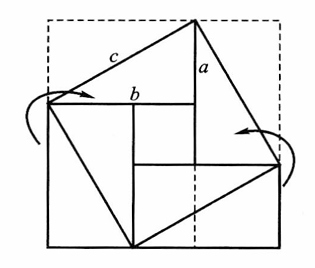
\includegraphics[scale=0.8]{"./Figures/string_graphic.png"}
    \caption{赵爽-弦图}
\end{figure}

\subsubsection{《九章算术》}
《九章算术》,成书于公元前1世纪前,由先秦至西汉中叶的长时期里经众多学者编纂、修改而成的一部重要的中国古典数学著作.

全书采用问题集的形式,共246个问题,分成九章,依次为:方田、粟米、衰分、少广、商功、均输、盈不足、方程、勾股. 
注重解决实际应用问题,其中所包含的数学成就是丰富和多方面的.

\begin{enumerate}
    \item 算术方面
    \begin{enumerate}
        \item 分数四则运算法则
        \item 比例算法
        \item 盈不足术
    \end{enumerate}
    \item 代数方面
    \begin{enumerate}
        \item 方程术(鸡兔同笼问题)
        \item 正负术(负数的引入)
        \item 开方术
    \end{enumerate}
    \item 几何方面
    \begin{enumerate}
        \item 精确的直线型几何图形的面积、体积公式(明确的算法)
    \end{enumerate}
\end{enumerate}

\subsection{从刘徽到祖冲之}
魏晋南北朝时期(公元220-公元581年),是中国思想相对活跃的时期,在长期独尊儒术之后,
数学的思辨之风再起,论证趋势出现.

这一时期的重要数学家有:赵爽,刘徽和祖冲之父子.

\subsubsection{刘徽的数学成就}
\textbf{刘徽(公元3世纪魏晋人)}: 生平不详(几乎没有任何文献记载这位大数学家的一生),创造了“割圆术”和体积理论.

\textbf{数学成就}:
\begin{itemize}
    \item 割圆术:通过圆的内接正多边形来计算圆的周长与面积,中国古代微积分思想的起源.
    \item 体积理论:通过“出入相补”原理,将几何图形分割成若干易于计算的部分计算总和.
    \begin{itemize}
        \item 构造一种新的几何图形“牟合方盖”,通过比例计算球的体积(虽然没有成功).
        \begin{figure}[H]
            \centering
            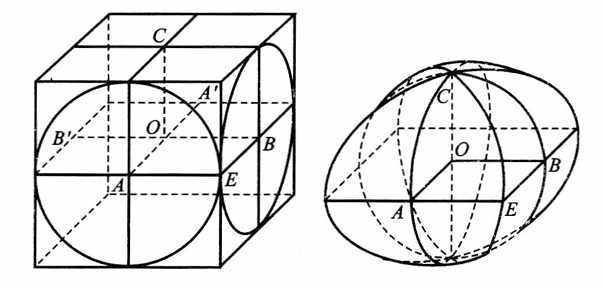
\includegraphics[scale=0.8]{"./Figures/LiHui_con_geo.png"}
            \caption{刘徽-牟合方盖}
        \end{figure}
    \end{itemize}
\end{itemize}

\subsubsection{祖冲之与祖暅}
\textbf{祖冲之(公元429-500)}:活跃于南朝宋、齐两代,出生于历法世家,代表作是《缀术》,与其子祖暅解决了诸多重要的数学问题.

\textbf{数学成就}:
\begin{itemize}
    \item 圆周率:沿用割圆术,计算出了圆周率数值的上下限:$3.1415926 \leq \pi \leq 3.1415927$
    \item 祖氏原理与球体积
    \begin{enumerate}
        \item 祖氏原理:幂(水平截面积)势(高)既容(相等),则积(体积)不容异.
        \item 球体积:祖暅延续刘徽的工作,计算了牟合方盖的体积,从而得到球的体积.
        \begin{figure}[H]
            \centering
            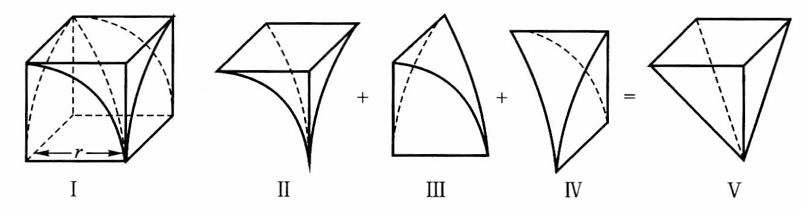
\includegraphics[scale=0.8]{"./Figures/LiuHui_con_geo_cal.png"}
            \caption{祖暅-计算牟合方盖($\frac{1}{8}$)的体积}
        \end{figure}
    \end{enumerate}
\end{itemize}

\subsubsection{《算经十书》}
隋唐开设的“算学”,选取十部算术经典作为数学教材,普及数学教育:
《周髀算经》,《九章算术》,《海岛算经》,《孙子算经》,《张邱建算经》,《夏侯阳算经》,《五曹算经》,《五经算术》,《缀术》,《缉古算经》.

\begin{enumerate}
    \item 孙子算经与“物不知数”问题:一次同余问题与孙子定理(中国剩余定理)\textit{(很难想象起名的历史学家的精神状态)}.
    \item 《张邱建算经》和“百鸡问题”:不定方程组问题.
    \item 《缉古算经》与三次方程:讨论了三次方程正根的数值解法.
\end{enumerate}

\subsection{宋元数学}
宋元时期(公元960年-1368年)的再次统一和印刷术等技术发明的出现,使得这一时期的中国古代数学有了再一次的卓越发展,并达到了顶峰.
\subsubsection{从“贾宪三角”到“正负开方”术}
宋元数学最突出的成就之一,高次方程数值求解,是《九章算术》开平方和开立方术的继承发展.

\begin{enumerate}
    \item 贾宪三角与增乘开方法:贾宪三角即杨辉三角(二项式系数三角塔),增乘开方法是一种用于求高次开方的算法.
    \item 秦九韶“正负开方术”:求解高次方程的迭代算法.
\end{enumerate}

\subsubsection{中国剩余定理}
用现代数学的语言来说明,中国剩余定理给出了以下的一元线性同余方程组:

\begin{equation}
    (S):\ \ \left\{\begin{array}{l l}{{x\equiv a_{1}\ \ (\mathrm{mod}\ \ m_{1})}}\\ {{x\equiv a_{2}\ \ (\mathrm{mod}\ \ m_{2})}}\\ 
        {{\vdots}}\\ {{x\equiv a_{n}\ \ (\mathrm{mod}\ \ m_{n})}}\end{array}\right.
\end{equation}

有解的判定条件,并用构造法给出了在有解情况下解的具体形式.

中国剩余定理说明:假设整数$m_{1},m_{2},\cdots,m_{n}$其中任意两数互质,则对任意的整数$a_{1},a_{2},\cdots,a_{n}$,方程组$\left(S\right)$有解,
并且通解可以由如下方式构造得到:

\begin{enumerate}
    \item 设$M=m_{1}\times m_{2}\times\cdots m_{n}=\prod_{i=1}^{n}m_{i}$是整数$m_{1},m_{2},\cdots,m_{n}$的乘积,并设
    $M_{i}=\frac{M}{m_{i}}, \forall i \in \left\{1,2,\cdots,n\right\}$,即$M_{i}$是除了$m_{i}$以外的$n-1$个整数的乘积.
    \item 设$t_{i}=M_{i}^{-1}$为$M_{i}$的数论倒数:$t_{i}M_{i}\equiv1{\quad}\mathrm{{(mod~}}m_{i}\mathrm{{),~}}{\forall i\in\{\![1,2,\cdots,n\}}$.
    \item 方程组$\left(S\right)$的通解形式为:$x=a_{1}t_{1}M_{1}+a_{2}t_{2}M_{2}+\cdots+a_{n}t_{n}M_{n}+k M=k M+\sum_{i=1}^{n}a_{i}t_{i}M_{i},\quad k\in\mathbb{Z}$.
\end{enumerate}

\subsubsection{内插法与垛积术}
问题背景:古代天算家由于编制历法,需要确定天体的视运动,而当他们观察出天体运动呈现不均匀性时,内插法便应运而生. 

\textbf{朱世杰(公元1300年前后)}:代表作由《算学启蒙》(1299)和《四元玉鉴》(1303),获得了一般高次内插公式.

\textbf{沈括(公元1031-1095)}:代表作《梦溪笔谈》,研究了高阶等差数列求和的公式“隙积术”.

朱世杰改进了沈括的求和公式并获得了普遍的高阶等差级数求和的一般公式:

\begin{equation}
    \begin{split}
        &\Sigma_{1}^{n} \frac{1}{p!}r\left(r+1\right)\left(r+2\right)\cdots\left(r+p-1\right) \\ 
        &= \frac{1}{(p+1)!}n\left(n+1\right)\left(n+2\right)\cdots\left(n+p\right)
    \end{split}
\end{equation}

\subsubsection{“天元术”与“四元术”}
高次方程及方程组数值解的求解技术. 主要人物有李治(公元1192-1279)、朱世杰.

%Chapter 5
\section{印度与阿拉伯数学}
\subsection{印度数学}
如果说希腊数学与其哲学密切相关,那么古代印度数学则更多地受到其宗教的影响.
雅利安人建立的婆罗门教(公元4世纪后改革为印度教),以及稍后(公元前6世纪)兴起的佛教、耆那教等,形成了古代印度数学发展的浓厚的宗教氛围.

印度数学的发展可以划分为3个重要时期:
\begin{itemize}
    \item 雅利安人入侵以前的达罗毗茶人时期(约公元前3000一前1400),史称河谷文化.
    \item 吠陀时期(约公元前10世纪一前3世纪).
    \item 悉檀多时期(5世纪一12世纪).
\end{itemize}

\begin{enumerate}
    \item 古代《绳法经》(公元前8世纪-前2世纪):记载了古印度一些建筑中的几何和代数计算问题.
    \item “巴克沙利手稿”(公元前2世纪-公元3世纪)与零号:其数学内容十分丰富,涉及分数、平方根、数列、收支与利润计算、比例算法、级数求和、代数方程等,
    其代数方程包括一次方程、联立方程组、二次方程. 特别值得注意的是手稿中使用了一些数学符号与今天的数学符号相似,以及出现了完整的十进制数码. 
    \item “悉檀多”时期的印度数学:印度数学的繁荣时期. 
    \begin{enumerate}
        \item 阿耶波多:《阿耶波多历数书》,改进了希腊三角学和一次不定方程的解法. 建立了Diophantus方程求解的所谓“Kuttaka方法”.
        \item 婆罗摩笈多:《婆罗摩修正体系》(628)和《肯德卡迪亚格》(约665),阐述了0的运算法则,以及给出了Pell方程的一种特殊解法.
        \item 马哈维拉:《计算方法纲要》,对以往数学内容的总结和推广,给出了一般性的组合数公式和椭圆周长近似公式.
        \item 婆什迦罗:《莉拉沃蒂》和《算法本源》,代表了古印度数学的最高水平.
    \end{enumerate}
\end{enumerate}

总结:由于印度屡被其他民族征服,使印度古代天文数学受外来文化影响较深,除希腊天文数学外,也不排除中国文化的影响,
然而印度数学始终保持东方数学以计算为中心的实用化特点.与算术和代数相比,印度人在几何方面的工作则显得薄弱.

\subsection{阿拉伯数学}
\subsubsection{阿拉伯的代数}
\begin{enumerate}
    \item \textbf{花剌子米《代数学》}
    \begin{itemize}
        \item \textbf{花剌子米(Mohammed ibn Musa al-Khawarizmi,约783-850)}:对欧洲数学影响最大的中世纪阿拉伯数学家.
        \item 《代数学》是花剌子米系列著作的统称,虽然其中的问题本身大部分相对Diophantus的著作和印度人的问题较为简单,但是因为
        花剌子米探讨了其中的一般性解法,因而更接近于近代初等代数. 对欧洲的数学教育和代数学发展起到了即为重要的作用. 
        \item 内容概览:《代数学》的数学问题都是由根($x$)、平方($x^{2}$)和数(常数)这三者组成. 接着分6章叙述6种类型的一、二次方程求解问题.
    \end{itemize}
    \item \textbf{奥马$\cdot$海亚姆与三次方程}
    \begin{itemize}
        \item \textbf{奥马$\cdot$海亚姆(Omar Khayyam,约1048-1131)}:11世纪最著名且最富有成就的数学家、天文学家和诗人. 
        \item 成就:制定了精密的历法——哲拉里历;开平方、开立方算法;以及最重要的圆锥曲线解三次方程. 
    \end{itemize}
\end{enumerate}

\subsubsection{阿拉伯的三角学和几何学}
由于数理天文学的需要,阿拉伯人继承并推进了希腊的三角术,其学术主要来源于印度的《苏利耶历数全书》等天文历表,
以及希腊托勒玫的《大成》、梅内劳斯的《球面学》等古典著作. 

正因为天文计算的需要,阿拉伯数学家致力于高精度的三角函数表的编制.

公元9世纪的海拜什$\cdot$哈西卜在印度人的基础上改进了正弦表和正切表;公元10世纪艾布$\cdot$瓦法在前者的基础上编制出了更为精确的间隔为$10^{'}$的
正弦表和余弦表;同时期晚些的比鲁尼利用二次插值制定了正弦、正切函数表;此外公元9世纪的天文学家阿尔$\cdot$巴塔尼系统总结了希腊三角学的结果,正是他
创立了系统的三角学术语(如正弦、余弦、正切、余切等),其天文著作更是影响了后来欧洲一代著名数学家.

此外,阿拉伯人对三角函数公式也有一定的研究(和印度人相似,大多都是算术性的);在几何方面,阿拉伯人主要对希腊时期的几何著作作了翻译与保存工作,并
传到了欧洲,不过阿拉伯人也在此过程中与古希腊几何产生了跨越时空的思想碰撞:较为突出的是不少该时期的数学家都试图证明《原本》中的第五公设,即平行公设,
诱导了后世欧洲学者在这方面的兴趣,间接影响了非欧几何的诞生. 

%Chapter 6
\section{近代数学的兴起}
\subsection{中世纪的欧洲}
中世纪的欧洲由于政治宗教原因,一直徘徊不前(几乎没有发展),直到公元12、13世纪的文艺复兴,欧洲数学才出现复苏发展的迹象. 

下图是古代学术传播西欧的路线:

\begin{figure}[H]
    \centering
    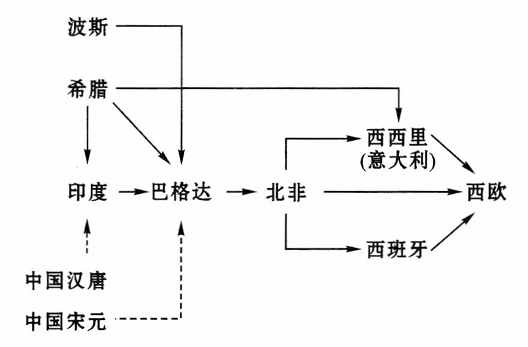
\includegraphics[scale=0.8]{"./Figures/Academia_spread_to_Euro.png"}
    \caption{古代学术传播西欧的路线}
\end{figure}

\textbf{斐波那契(L.Fibonacci, 1170-1250)}: 文艺复兴初期第一位有影响的数学家,早年在北非师从阿拉伯人并游历地中海沿岸诸国,
后编著了古代中国、印度和希腊的数学问题集《算经》. 其中记载有著名的Fibonacci兔子数列.

\subsection{向接近代数学的过渡}
\subsubsection{代数学}
1515年,波伦亚大学的数学教授费罗(S.Ferro, 1465-1526)发现了形如$x^{3}+mx=n (m,n \geq 0)$的三次方程的代数解法.
按照当时的风气,费罗将自己的解法秘密传授给了他的学生费奥(A.M.Fior)

1535年,意大利的一位数学家塔塔利亚(Niccolo Fontana, 1499?-1557, 绰号Tartaglia意为口吃者),发现了解形如$x^{3}+mx^{2}=n (m,n \geq 0)$的三次方程的解法.

后来另一位米兰学者卡尔丹从塔塔利亚学到了这他的解法,并在1545年出版的著作《大法》(Ars Magna)中公布了它们. 
进一步地,卡尔丹发现对于带有二次项的三次方程,总可以通过变换将二次项消去,化为$x^{3}=px+q$的形式.

三次方程解决不就后,1540年意大利数学家达科伊(T.da Coi)向卡尔丹提出了一个四次方程的问题,该问题由其学生费拉里(L.Ferrari, 1522-1565)所解决,其解法被收录于《大法》中.

卡尔丹等人在求解多项式方程的根时,已经意识到复数的存在以及复根总是成对存在的. 在卡尔丹的基础上荷兰人吉拉德(A.Girard, 1593-1632)于《代数新发现》(1629)中
又对多项式的根与次数的关系作了进一步的推断,即著名的“代数基本定理”.

此外,卡尔丹还发现三次方程的根与系数有一定的关系,这种具体的结果后来由韦达、牛顿和格里戈里(J.Gregory, 1638-1675)等人作出系统阐述. 

法国数学家韦达(F.Vieta, 1540-1603)创作了《分析引论》(In Artem Analyticem Isagoge, 1591)、《论方程的整理与修正》(1615)等方程论著作,给出代数方程的近似解法
与代数方程的多项式分解因式解法. 1637年,笛卡儿首次应用待定系数法将四次方程分解成两个二次方程求解. 今天所说的因式分解定理,最早由笛卡儿在其《几何学》中提出. 

代数上的进步还在于引用了较好的符号体系,而这主要归功于韦达和笛卡尔的工作. 

\subsubsection{三角学}
由于航海、历法推算以及天文观测的需要,三角学得以进一步发展.

从早期的球面三角到平面三角学:波伊尔巴赫(G.Peurbach, 1423-1461),编译了十分精确的正弦表;他的学生雷格蒙塔努斯(J.Regiomontanus, 1436-1476)写了
第一部脱离了天文学的三角学专著. 哥白尼的学生雷提库斯(G.J.Rhaeticus, 1514-1576)将传统的弧与弦的关系,改进为角的三角函数关系,并采用了六个函数.

三角学的进一步发展来自于韦达所做的平面三角与球面三角系统化工作.

\subsubsection{从透视学到射影几何}
早期,意大利人布努雷契(F.Brunelleschi, 1377-1446)和法国自学成才的工程师德沙格(G.Desargues, 1591-1661),开始研究投影与透视背后的数学原理.

后来,法国数学家帕斯卡(B.Pascal, 1623-1662)受德沙格的建议,简化了圆锥曲线的诸多性质,创作了《圆锥曲线论》,提出了著名的Pascal定理:
圆锥曲线的内接六边形对边交点共线. 

此外还有画家出身拉伊尔(P.de La Hire, 1640-1718)也受到了德沙格的影响,用投影的思想证明了诸多圆锥曲线的定理,并在极点理论方面有所创新. 

\subsubsection{计算技术与对数}
16世纪前半叶,这一时期计算技术最大的改进是对数的发明和应用,它的产生主要是由于天文和航海计算的强烈需要. 为简化天文、航海方面
所遇到的繁杂数值计算,自然希望将乘除法归结为简单的加减法. 

苏格兰贵族数学家纳皮尔(J.Napier, 1550一1617)正是在球面天文学的三角学研究中首先发明对数方法的.1614年他在题为《奇妙的对数定理
说明书》的小书中,阐述了他的对数方法. 

\subsection{解析几何的诞生}
近代数学本质上说可以看作变量数学,而变量数学的第一个里程碑是解析几何的发明. 

解析几何的基本思想:在平面上引进所谓的“坐标”的概念,并借助这种坐标在平面上的点和有序数对$(x,y)$之间建立一一对应的关系.

解析几何的真正发明要归功于法国另外两位数学家笛卡儿(R.Descartes,1596一1650)与费马(P.de Fermat,1601一1665).他们工作的出发点不同,但却殊途同归.

%Chapter 7
\section{微积分的创立}
微积分的思想萌芽,特别是积分学,部分可以追溯到古代. 我们已经知道,面积和体积的计算自古以来一直是数学家们感兴趣的课题,在
古代希腊、中国和印度数学家们的著述中,不乏用无限小过程计算特殊形状的面积、体积和曲线长的例子.前面已经介绍过阿基米德、刘徽和
祖冲之父子等人的方法,他们的工作,确实是人们建立一般积分学的漫长努力的先驱.

与积分学相比而言,微分学的起源则要晚得多.刺激微分学发展的主要科学问题是求曲线的切线、求瞬时变化率以及求函数的极大极小值等问题. 

\subsection{半个世纪的酝酿}
近代微积分的酝酿,主要是在17世纪上半叶这半个世纪.

1608年,荷兰眼镜制造商里帕席发明了望远镜,不久伽利略将他制成的第一架天文望远镜对准星空而作出了令世人目不暇接、惊奇不已的天文发现.

1619年,开普勒公布了他的最后一条行星运动定律.开普勒行星. 运动三大定律要意是:

\begin{enumerate}
    \item 行星运动的轨道是椭圆,太阳位于该椭圆的一个焦点. 
    \item 由太阳到行星的矢径在相等的时间内扫过的面积相等. 
    \item 行星绕太阳公转周期的平方,与其椭圆轨道的半长轴的立方成正比. 
\end{enumerate}

1638年,伽利略(Galileo Galilei, 1564-1642)建立了自由落体定律、动量定律等. 

此外,一系列微分学问题成为人们关注的焦点:瞬时变化率问题;切线问题;函数极大值、极小值问题;面积、体积、曲线长、重心和引力计算问题.

不少数学家在相关领域也做了许多重要工作:

\begin{enumerate}
    \item 开普勒与旋转体体积
    \item 卡瓦列里不可分量原理
    \item 笛卡尔“圆法”
    \item Fermat求极值的方法
    \item 巴罗“微分三角形”
    \item 沃利斯“无穷算术”
\end{enumerate}

\subsection{牛顿的“流数术”}

牛顿(Isaac Newton, 1642-1727)于伽利略去世那年一1642年(儒略历)的圣诞出生于英格兰林肯郡伍尔索普村一个农民家庭. 

牛顿对微积分问题的研究始于1664年秋,当时他反复阅读笛卡儿《几何学》,对笛卡儿求切线的“圆法”发生兴趣并试图寻找更好的方法.就在此时,牛顿首创了小$o$记号表示$x$的无限小且最终趋于零的增量.

1665年夏至1667年春,牛顿在家乡躲避瘟疫期间,继续探讨微积分并取得了突破性进展.据他自述,1665年11月发明“正流数术”(微分法),次年5月又建立了“反流数术”(积分法).
1666年10月,牛顿将前两年的研究成果整理成一篇总结性论文,此文现以《流数简论》(Tract on Fluxions)著称,当时虽未正式发表,但在同事中传阅.《流数简论》(以下简称《简论》)是历史上第一篇系统的微积分文献.

《流数简论》反映了牛顿微积分的运动学背景.该文事实上以速度形式引进了“流数”(即微商)概念.

1667年春,牛顿回到剑桥,并在此后约四分之一世纪的时间里,始终不渝努力改进、完善自己的微积分学说,先后写成了三篇微积分论文,它们分别是:

\begin{enumerate}
    \item 《运用无限多项方程的分析》(De Analysi per Aequationes Numero Terminorum Infinitas,简称《分析学》,完成于l669年). 
    \item 《流数法与无穷级数》(Methodus Fluxionum et Serierum Infinitarum,简称《流数法》,完成于1671年). 
    \item 《曲线求积术》(Tractatus de Quadratura Curvarum,简称《求积术》,完成于1691年).
    \item 力学名著《自然哲学的数学原理》(Philosophiae naturalis principia mathematica,以下简称《原理》),出版于1687年,最早公开表述牛顿微积分的著作. 
\end{enumerate}

从上述文章中可以寻得牛顿对微分思想和积分思想的理解与阐述,供感兴趣的同学参考.

实际上微积分的思想非常的简单,任何一位学习过《微积分》课程的同学都应该清楚地认识到这一思想在解决实际问题以及进一步的物理问题时的实际用法. 我们非常推荐大家去找一道有意思的数学或者物理问题,
用微分的思想刨析它、再用积分的方法解决它(或者反过来),这样才能深刻理解微积分的内涵. 

\subsection{莱布尼茨的微积分}
在微积分的创立上,牛顿需要与莱布尼茨分享荣誉. 

莱布尼茨(Gottfried Wilhelm Leibniz,1646一1716)出生于德国莱比锡的一个教授家庭. 早年在莱比锡大学学习法律,同时开始接触伽利略、
开普勒、笛卡儿、帕斯卡以及巴罗等人的科学思想. 

莱布尼茨在微积分方面,莱布尼茨和牛顿的工作大同小异,唯一的区别是莱布尼茨创造并改进了微积分的符号(如我们熟知的积分符号$\int$就是由莱布尼茨发明的)且更加注重微积分的解析运算(这一点或许可以与牛顿有所区别,因为在
Leibniz的著作中,主要以解析式和文字居多,而牛顿的原理对微积分的解释最初大多以图片形式呈现). 

莱布尼茨的博学多才在科学史上罕有所比,其著作涉及数学、力学、机械、地质、逻辑、哲学、法律、外交、神学和语言学等.在数学上,他的贡献也远不止微积分.

莱布尼茨在l666年发表的《组合艺术》(De Arte Combinatoria)和一些相关的文稿中,提出了符号逻辑的思想,引导了布尔、罗素等人的数理逻辑.

莱布尼茨1679年撰写的《二进制算术》,使他成为二进记数制的发明人·二进制在现代被应用于计算机设计,但莱布尼茨本人并没有将它用到自己的计算机上.莱布尼茨后来发现他的二进制数可以给中国
古老的六十四卦易图一个很好的数学解释,他是通过他的朋友、法国传教士白晋(F.J.Bouvet)得到六十四卦图的.莱布尼茨高兴地说:“可以让我加入中国籍了吧”!

\subsection{牛顿与莱布尼茨}
牛顿和莱布尼茨都是他们时代的巨人.就微积分的创立而言,尽管在背景、方法和形式上存在差异、各有特色,但二者的功绩是相当的. 
他们都使微积分成为能普遍适用的算法,同时又都将面积、体积及相当的问题归结为反切线(微分)运算. 应该说,微积分能成为独立的
科学并给整个自然科学带来革命性的影响,主要是靠了牛顿与莱布尼茨的工作. 在科学史上,重大的真理往往在条件成熟的一定时期由
不同的探索者相互独立地发现,微积分的创立,情形也是如此. 

%Chapter 8
\section{分析时代}
本章主要讨论了分析时代的数学发展,涵盖了微积分的发展、微积分的应用与新分支的形成,以及18世纪的几何与代数。
\subsection{微积分的发展}
\begin{itemize}
    \item \textbf{伯努利家族}
    \begin{itemize}
        \item \textbf{雅各布·伯努利(Jakob Bernoulli, 1654-1705)}:
        \begin{itemize}
            \item 主要著作:《无穷级数研究》、《概率论》
            \item 贡献:研究了无穷级数、常微分方程和概率论,对数学分析的发展有重要影响。
        \end{itemize}
        \item \textbf{约翰·伯努利(Johann Bernoulli, 1667-1748)}:
        \begin{itemize}
            \item 主要著作:《积分法》、《变分法研究》
            \item 贡献:在微分方程和变分法方面有重要贡献。
        \end{itemize}
    \end{itemize}
    
    \item \textbf{欧拉(Leonhard Euler, 1707-1783)}:
    \begin{itemize}
        \item 主要著作:《无穷小分析引论》、《微积分学》、《纯粹分析》
        \item 贡献:在微积分、拓扑学和图论等多个领域做出了卓越贡献,引入了许多重要的数学概念和记号,如 $e^{i\pi} + 1 = 0$ 以及函数符号 $f(x)$。
    \end{itemize}

    \item \textbf{微积分深入发展的几个重要方面}:
    \begin{enumerate}
        \item \textbf{级数的汇合与发散}
        \item \textbf{幂级数和傅里叶级数}
        \item \textbf{微分方程}
    \end{enumerate}
\end{itemize}

\subsection{微积分的应用与新分支的形成}
\begin{itemize}
    \item \textbf{拉格朗日(Joseph-Louis Lagrange, 1736-1813)}:
    \begin{itemize}
        \item 主要著作:《分析力学》、《数论》
        \item 贡献:在力学、分析和数论方面有重要贡献,创立了拉格朗日力学,提出了拉格朗日方程。
    \end{itemize}
    
    \item \textbf{拉普拉斯(Pierre-Simon Laplace, 1749-1827)}:
    \begin{itemize}
        \item 主要著作:《天体力学概论》、《概率论的解析理论》
        \item 贡献:在概率论和天体力学方面做出了杰出贡献,提出了拉普拉斯方程,研究了拉普拉斯变换。
    \end{itemize}

    \item \textbf{微积分的新分支}:
    \begin{enumerate}
        \item \textbf{变分法}
        \item \textbf{多元函数的微积分}
        \item \textbf{偏微分方程}
    \end{enumerate}
\end{itemize}

\subsection{18世纪的几何与代数}
\begin{itemize}
    \item \textbf{蒙日(Gaspard Monge, 1746-1818)}:
    \begin{itemize}
        \item 主要著作:《画法几何》
        \item 贡献:创立了画法几何,这不仅是一种数学方法,还成为工程设计的重要工具。
    \end{itemize}
    
    \item \textbf{达朗贝尔(Jean le Rond d'Alembert, 1717-1783)}:
    \begin{itemize}
        \item 主要著作:《力学》、《百科全书》
        \item 贡献:在微分方程和动力学方面有重要贡献,提出了达朗贝尔原理。
    \end{itemize}
    
    \item \textbf{几何与代数的发展}:
    \begin{enumerate}
        \item \textbf{解析几何的进一步发展}
        \item \textbf{代数方程的求解}
        \item \textbf{几何学与拓扑学}
    \end{enumerate}
\end{itemize}

%Chapter 9
\section{代数学的新生}
本章主要讨论了代数学在17至18世纪的复兴与发展,涵盖了代数学基础的奠定、代数学理论的进展,以及代数方程的求解与应用。

\subsection{代数学基础的奠定}
\begin{itemize}
    \item \textbf{笛卡尔(René Descartes, 1596-1650)}:
    \begin{itemize}
        \item 主要著作:《几何学》
        \item 贡献:创立了解析几何,将代数与几何结合起来,为代数学的发展奠定了基础。
    \end{itemize}
    
    \item \textbf{费马(Pierre de Fermat, 1601-1665)}:
    \begin{itemize}
        \item 主要著作:《费马大定理》
        \item 贡献:提出了数论中的许多重要命题,对后来的代数和数论研究产生了深远影响。
    \end{itemize}
    
    \item \textbf{牛顿(Isaac Newton, 1643-1727)}:
    \begin{itemize}
        \item 主要著作:《自然哲学的数学原理》、《广义二项式定理》
        \item 贡献:在二项式定理、无穷级数和代数方程求解方面做出了重要贡献。
    \end{itemize}
\end{itemize}

\subsection{代数学理论的进展}
\begin{itemize}
    \item \textbf{欧拉(Leonhard Euler, 1707-1783)}:
    \begin{itemize}
        \item 主要著作:《代数学引论》、《数论》
        \item 贡献:在复数理论、对数函数和数论等多个领域做出了卓越贡献,丰富了代数学的理论体系。
    \end{itemize}
    
    \item \textbf{拉格朗日(Joseph-Louis Lagrange, 1736-1813)}:
    \begin{itemize}
        \item 主要著作:《代数学讲义》、《方程的解》
        \item 贡献:在方程理论和代数解法方面有重要贡献,提出了拉格朗日乘数法。
    \end{itemize}
    
    \item \textbf{高斯(Carl Friedrich Gauss, 1777-1855)}:
    \begin{itemize}
        \item 主要著作:《算术研究》
        \item 贡献:在数论、代数几何和复数理论方面有卓越贡献,被誉为“数学王子”。
    \end{itemize}
\end{itemize}

\subsection{代数方程的求解与应用}
\begin{itemize}
    \item \textbf{拉普拉斯(Pierre-Simon Laplace, 1749-1827)}:
    \begin{itemize}
        \item 主要著作:《概率论的解析理论》、《天体力学概论》
        \item 贡献:研究了概率论和微分方程,提出了拉普拉斯方程和拉普拉斯变换。
    \end{itemize}
    
    \item \textbf{柯西(Augustin-Louis Cauchy, 1789-1857)}:
    \begin{itemize}
        \item 主要著作:《复变函数论》、《代数学》
        \item 贡献:在复分析和代数学方面有重要贡献,提出了柯西积分公式和柯西不等式。
    \end{itemize}

    \item \textbf{代数方程的求解方法}:
    \begin{enumerate}
        \item \textbf{拉格朗日乘数法}
        \item \textbf{高斯消元法}
        \item \textbf{复数解法}
    \end{enumerate}
\end{itemize}

%Chapter 10
\section{几何学的变革}
本章探讨了几何学在17至19世纪的重大变革,涵盖了解析几何、非欧几何的兴起和拓扑学的发展。

\subsection{欧几里得平行公设}
\begin{itemize}
    \item \textbf{欧几里得(Euclid, 公元前325-公元前265)}:
    \begin{itemize}
        \item 贡献:提出了平行公设,即在平面上,通过已知点只能作一条直线与已知直线平行。
        \item 主要著作:《几何原本》
    \end{itemize}
\end{itemize}


\subsection{解析几何的发展}
\begin{itemize}
    \item \textbf{笛卡尔(René Descartes, 1596-1650)}:
    \begin{itemize}
        \item 贡献:创立了解析几何,将代数方法应用于几何问题,建立了坐标系的概念。
        \item 主要著作:《几何学》
    \end{itemize}
    
    \item \textbf{费马(Pierre de Fermat, 1601-1665)}:
    \begin{itemize}
        \item 贡献:独立于笛卡尔发展了解析几何,提出了早期的坐标几何思想。
        \item 主要著作:《费马定理》
    \end{itemize}
\end{itemize}

\subsection{非欧几何的兴起}
\begin{itemize}
    \item \textbf{高斯(Carl Friedrich Gauss, 1777-1855)}:
    \begin{itemize}
        \item 贡献:提出了高斯曲率的概念,为非欧几何奠定了基础。
        \item 主要著作:《算术研究》
    \end{itemize}
    
    \item \textbf{罗巴切夫斯基(Nikolai Lobachevsky, 1792-1856)}:
    \begin{itemize}
        \item 贡献:创立了非欧几何学,即双曲几何。
        \item 主要著作:《几何学原理》
    \end{itemize}
    
    \item \textbf{黎曼(Bernhard Riemann, 1826-1866)}:
    \begin{itemize}
        \item 贡献:提出了黎曼几何,开创了多维空间的研究。
        \item 主要著作:《论几何基础》
    \end{itemize}
\end{itemize}

\subsubsection*{非欧几何的具体研究例子}
\begin{enumerate}
    \item \textbf{双曲几何的研究}:
    \begin{itemize}
        \item 罗巴切夫斯基对平行公理的替代
        \item 高斯的曲率概念应用
    \end{itemize}
    \item \textbf{椭圆几何的研究}:
    \begin{itemize}
        \item 黎曼的椭圆几何模型
    \end{itemize}
\end{enumerate}

\subsection{拓扑学的发展}
\begin{itemize}
    \item \textbf{欧拉(Leonhard Euler, 1707-1783)}:
    \begin{itemize}
        \item 贡献:解决了柯尼斯堡七桥问题,奠定了拓扑学的基础。
        \item 主要著作:《七桥问题》
    \end{itemize}
    
    \item \textbf{柯西(Augustin-Louis Cauchy, 1789-1857)}:
    \begin{itemize}
        \item 贡献:在分析学和拓扑学方面做出了重要贡献。
        \item 主要著作:《复变函数论》
    \end{itemize}
    
    \item \textbf{庞加莱(Henri Poincaré, 1854-1912)}:
    \begin{itemize}
        \item 贡献:被誉为拓扑学之父,提出了庞加莱猜想。
        \item 主要著作:《分析延展》
    \end{itemize}
\end{itemize}

\subsubsection*{拓扑学的重要成果}
\begin{enumerate}
    \item \textbf{柯尼斯堡七桥问题的解决}:
    \begin{itemize}
        \item 欧拉的拓扑学方法
    \end{itemize}
    \item \textbf{庞加莱猜想}:
    \begin{itemize}
        \item 庞加莱对三维空间拓扑结构的研究
    \end{itemize}
\end{enumerate}

\end{document}
